\begin{figure}[ht]
    \centering
    % 裁剪图片边缘可能存在的白色区域（根据实际情况调整参数）
        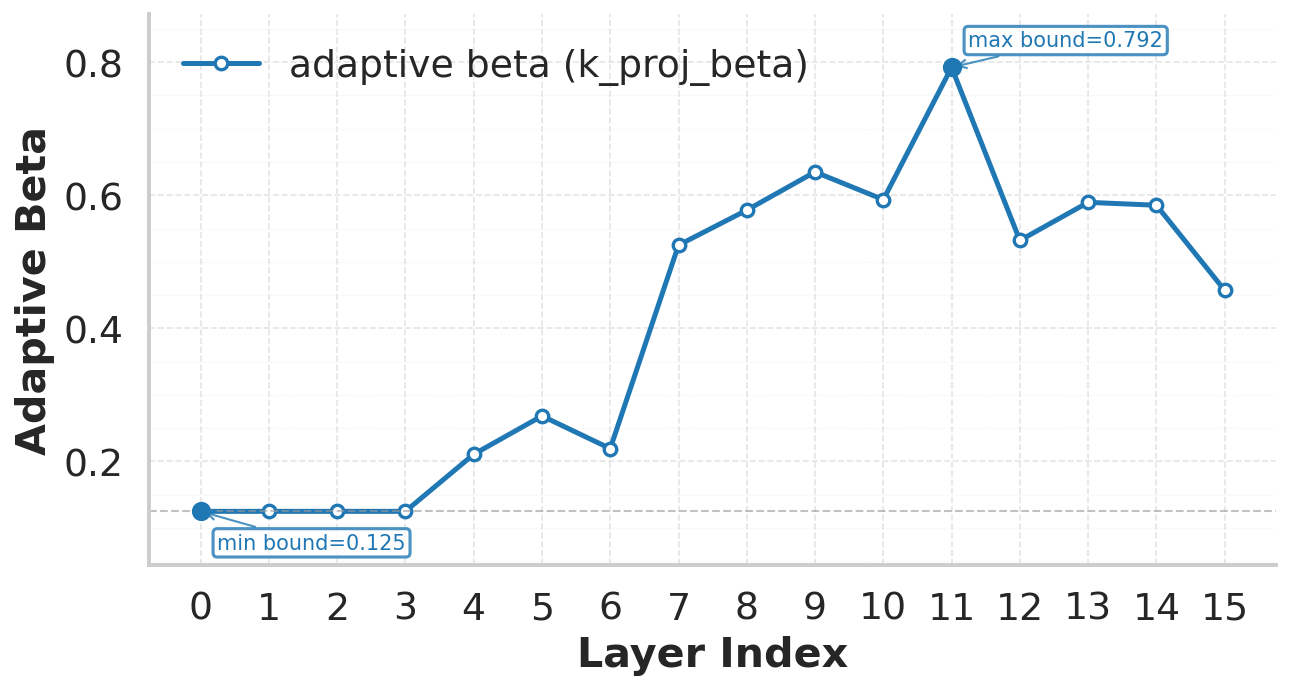
\includegraphics[width=1\linewidth]{figs/adaptive_beta_by_layer.png}
    % 调整标题与图片的距离
    \caption{The visualization of the optimal beta values obtained from k-proj of odd-numbered layers on LLaMA2-7B.}
    \label{fig:optiminal beta}  % 标签使用冒号分隔符，符合LaTeX规范
    % 调整图与下文的距离
    \end{figure}